\chapter{Background}
\label{Chapter2}
% Main chapter title
\lhead{Chapter 2. \emph{Background}}


This chapter introduces the background and terminology necessary to understand the concepts and methods presented in this thesis. Important terms are explained in corresponding sections.

As majority of web applications' functionality is accessed through the GUI layer, it becomes customary to test important functional use-cases on the AUT through the GUI layer. Section \ref{sec:AutomatedGUITesting} gives a brief insight into automated GUI testing mechanisms.

In recent years, Selenium\footnote{\url{http://www.seleniumhq.org/}} has been a popular browser test automation tool of choice among software developers and testers. Section\ref{sec:SeleniumTesting} gives the necessary background about Selenium framework, including its implementation techniques as well as salient features.

This research leverages existing Selenium tests to capture the behavior of the AUT in terms of finite state models. For this purpose, the tool \texttt{webmate}, presented by Dallmeier et al.\cite{webmate} has been used. By leveraging existing Selenium tests, \texttt{webmate} can systematically explore the AUT to extract its behavioral usage model by implementing state-abstraction for comparing similar GUI states of the AUT. Further details about \texttt{webmate} are discussed in Section \ref{sec:WebMate}

Section \ref{sec:Statistical} presents the statistical background required to analyze the results and apply the evaluation metrics, as presented in Chapter \ref{Chapter6}.

\section{Automated GUI Testing}
\label{sec:AutomatedGUITesting}
As mentioned in Section 1, testing web applications at GUI level abstracts away finer grained internal details and helps developers to identify the undesired functionality changes in the AUT.  In comparison to traditional command-line applications or Application Programming Interfaces (APIs), automated GUI testing of modern web 2.0 applications built with multiple languages, platforms and server-side technologies poses new challenges in the areas of test-input generation, test-output verification and state space exploration.

To begin with, automatically generating and selecting inputs for a GUI is difficult since depending upon the type of the application, different applications might require specific combinations of inputs and values. 
Current practices for automated test input generation include techniques such as symbolic execution\cite{Ganovetal}, using random input generation\cite{godefroid2005dart} or search based techniques\cite{gross2012search}. However, automated input generation is not trivial for a web applications, since the GUI test automation tool needs to be aware of the context of the AUT. Although test inputs can be generated using functional specifications, concrete specifications along with different input combinations may not be available in practice and desired functional coverage of the AUT is not achieved. Thus in many cases, input generation is often left to the test developer to explore the desired states of the AUT hidden behind input forms and elements.

In addition, even in cases when a testing tool can generate different input combinations automatically, it still needs to verify the correct behavior of the AUT. This is usually done by applying appropriate test assertions and oracles on the test outputs\cite{Baresi:Oracles}. Mechanisms such as using Capture/replay tools\cite{joshi2006capture} require the tester to first manually capture the behavior of the AUT by performing different GUI-level events, recording them and storing the expected output as a part of the test-case. In the replay phase, recorded tests are replayed on the AUT and the output is checked against the captured textit{expected output} to assert the application behavior. Such approach requires manual effort to record each test and is not suitable for regression testing as every time the AUT changes, there is a need to re-record the tests in order to generate new expected outputs. 

Moreover, as the size of the AUT increases, the number of possible actions on the GUI increases exponentially. This is especially an issue in case of regression testing since as possible number of paths and sequences increases, covering the entire possible number of state space and executions becomes infeasible.

On the other hand, as opposed to the automated crawlers, humans possess the domain knowledge of the AUT required to generate valid test inputs and apply precise oracles on the test outputs, many developers often choose to identify the core functionality of the AUT and automate their regression tests using frameworks such as Selenium, as detailed in Section 2.2.

\section{Test automation using Selenium}
\label{sec:SeleniumTesting}
\subsection{Selenium WebDriver}
Selenium is a browser automation framework designed to automate the system testing of web applications. While the Selenium project offers a different set of tools depending upon the type of application, the  \texttt{webdriver}\footnote{\url{http://www.seleniumhq.org/projects/webdriver/}} project is of particular the interest for laying the foundation of this thesis. The \texttt{webdriver} project provides an API to test dynamic web 2.0 applications. The API \textit{drives} (controls) the browser in a manner that it emulates all possible end users interactions with the browser, such as clicks, form-inputs, drag-drops, file up- loads etc. Selenium \texttt{webdriver} tests can thus explore the possible set of functionalities of the AUT 

The \texttt{webdriver} API supports various modern programming languages such as Java, Python, C\#, Ruby, PHP etc. by providing language level bindings along with a set of browser specific drivers. Figure \ref{fig:webdriverArchitecture} gives an overview of the architecture of Selenium \texttt{webdriver}.
 
\begin{figure}[h!]
\makeatletter 
% \renewcommand{\thefigure}{\@arabic\c@figure}
\makeatother
    \centering
  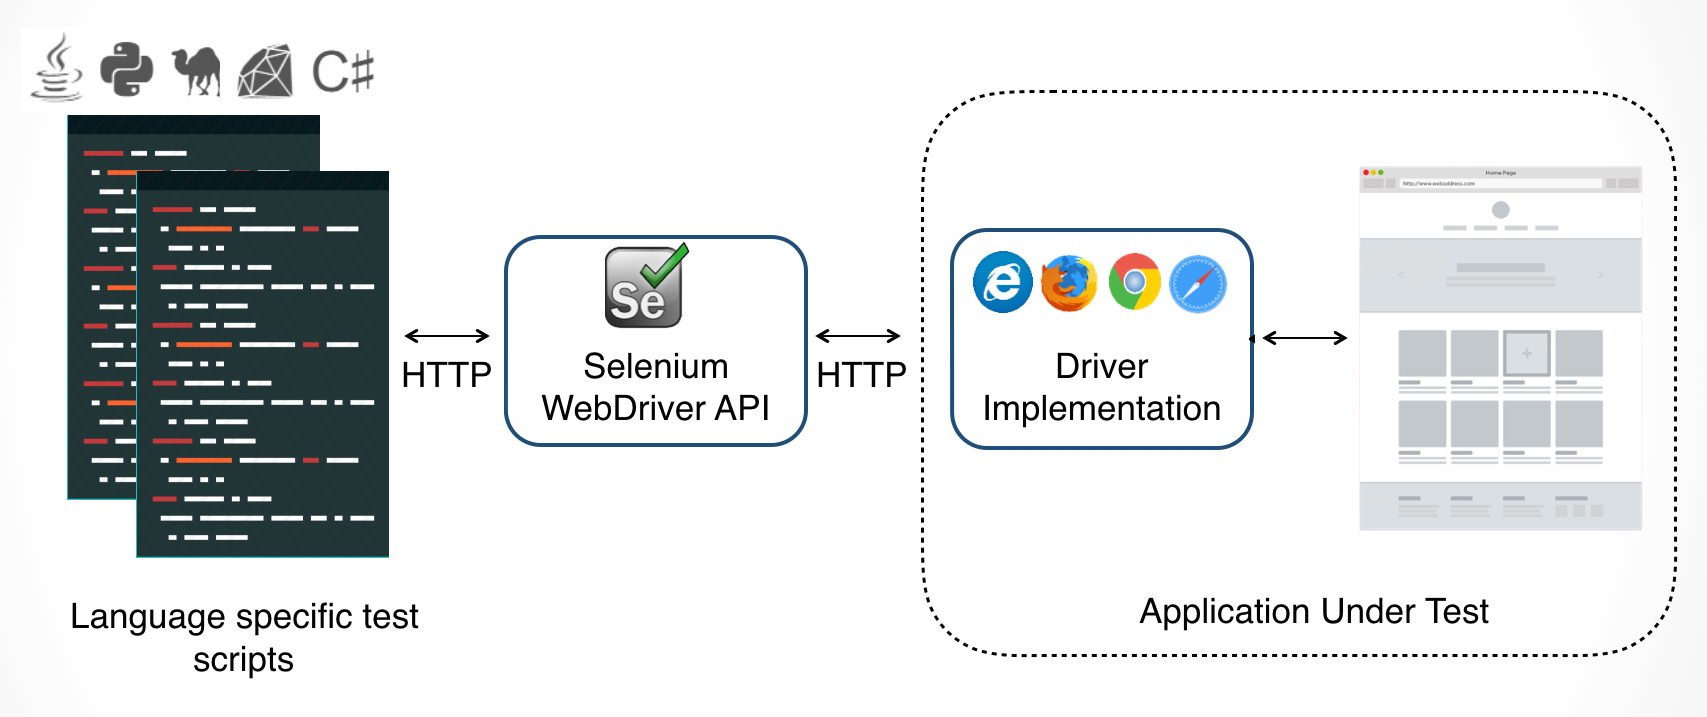
\includegraphics[width=5.5in,height=2.2in]{./Figures/webdriver_Archi}
  \caption{Selenium \texttt{webdriver} architecture}
  \label{fig:webdriverArchitecture} 
\end{figure}

The \texttt{webdriver} API communicates with the browser specific driver using a common wire protocol. The protocol transfers the test-commands written in language specific bindings to the browser specific driver in the form of UTF-8\footnote{\url{https://tools.ietf.org/html/rfc3629}} encoded JSON\footnote{\url{http://www.json.org/}} data. The API uses HTTP\footnote{\url{https://www.w3.org/Protocols/}} as a transport mechanism to transfer these commands to the driver and to return the response from the driver to the language specific code. 

Each browser specific driver implementation such as the \texttt{Firefox Driver}\footnote{\url{https://code.google.com/p/selenium/wiki/FirefoxDriver}} or the \texttt{RemoteWebDriver}\footnote{\url{https://code.google.com/p/selenium/wiki/RemoteWebDriver}} has its own mechanism for carrying out the above-mentioned communication. 

The \texttt{RemoteWebDriver} implementation provides the capability to run the Selenium tests against a remote machine. In essence, \texttt{RemoteWebDriver} is comprised of a client-server architecture, where client is the language specific test-case and and server is a simple Java servlet. The \texttt{RemoteWebDriver} servlet acts as a multiplexer, by connecting the client to the specific browser(s) and system configurations requested by the client. The browser and other configurations are provided in terms of capabilities, via command-line or directly from the language specific code. \\

\noindent 
Following example illustrates the communication between the language specific test-commands (Java in this case) and the \texttt{RemoteWebDriver} through \texttt{webdriver} API :
\begin{enumerate}
\item The client (test-script) requests the URL of the AUT. 
\begin{verbatim}
driver.get("http://www.application-under-test.com");
\end{verbatim}
\item This command is translated as a JSON object to be transferred using the wire protocol as following: 
\begin{verbatim}
{"url": "http://www.application-under-test.com" }
\end{verbatim}
\item The JSON object is then sent over HTTP (using POST\footnote{\url{http://tools.ietf.org/html/rfc7231\#section-4.3.3}} request in this case). To identify and associate each request/response session uniquely to the session-specific commands, \texttt{webdriver} uses a unique handle in terms of the \textit{SessionId}
\begin{verbatim}
HTTP Method : POST, Path: session/{session-id}/url
\end{verbatim}
The resultant URL is :
\begin{verbatim}
http://localhost:7055/hub/session/{session-id}/url
\end{verbatim}
\end{enumerate}

In order to locate GUI elements such as input forms, buttons, checkboxes etc. in the DOM (Document Object Model), Webdriver specifies "Find Element" and "Find Elements" methods for locating a single element and a list of elements, respectively. Each language specific binding has its own command to invoke these methods by providing the UI locator object, such as the css selector or xpath expression. The the element locator strategies are listed in TABLE XXX. As we will see in CHAPTER XXX ROBUSTNESS, influence of these UI locator strategies is discussed 
% (https://w3c.github.io/webdriver/webdriver-spec.html#sessions)

\section{WebMate}
\label{sec:WebMate}
WebMate is a system-level automated testing and analysis framework. It can leverage existing Selenium tests in order to remote control the browser to interact with the dynamic web 2.0 applications involving JavaScript and Ajax elements. By doing so, it can systematically explore the AUT in order to extract its behavioral usage-model. To do so, it implements state abstraction in order to distinguish similar GUI states of the AUT. The usage model is a finite state automaton, which captures the exploration graph of the possible ways to interact with the AUT. The states of the behavioral model correspond to different states of the GUI, connected by transitions corresponding to different interactions with the AUT. 
To this date, WebMate primarily functions for checking cross-browser compatibility. It can detect functional as well as GUI differences across the browsers. WebMate is able to identify the GUI elements and compare their positions, sizes and inconsistencies across the GUIs to generate a report visualizing the differences. Moreover, WebMate makes it possible to recognize functional differences (e.g. missing button) by comparing the usage models and presenting the XPath representation of the changed element

\section{Statistical Background}
\label{sec:Statistical}